\documentclass[twoside]{book}

% Packages required by doxygen
\usepackage{fixltx2e}
\usepackage{calc}
\usepackage{doxygen}
\usepackage[export]{adjustbox} % also loads graphicx
\usepackage{graphicx}
\usepackage[utf8]{inputenc}
\usepackage{makeidx}
\usepackage{multicol}
\usepackage{multirow}
\PassOptionsToPackage{warn}{textcomp}
\usepackage{textcomp}
\usepackage[nointegrals]{wasysym}
\usepackage[table]{xcolor}

% Font selection
\usepackage[T1]{fontenc}
\usepackage[scaled=.90]{helvet}
\usepackage{courier}
\usepackage{amssymb}
\usepackage{sectsty}
\renewcommand{\familydefault}{\sfdefault}
\allsectionsfont{%
  \fontseries{bc}\selectfont%
  \color{darkgray}%
}
\renewcommand{\DoxyLabelFont}{%
  \fontseries{bc}\selectfont%
  \color{darkgray}%
}
\newcommand{\+}{\discretionary{\mbox{\scriptsize$\hookleftarrow$}}{}{}}

% Page & text layout
\usepackage{geometry}
\geometry{%
  a4paper,%
  top=2.5cm,%
  bottom=2.5cm,%
  left=2.5cm,%
  right=2.5cm%
}
\tolerance=750
\hfuzz=15pt
\hbadness=750
\setlength{\emergencystretch}{15pt}
\setlength{\parindent}{0cm}
\setlength{\parskip}{3ex plus 2ex minus 2ex}
\makeatletter
\renewcommand{\paragraph}{%
  \@startsection{paragraph}{4}{0ex}{-1.0ex}{1.0ex}{%
    \normalfont\normalsize\bfseries\SS@parafont%
  }%
}
\renewcommand{\subparagraph}{%
  \@startsection{subparagraph}{5}{0ex}{-1.0ex}{1.0ex}{%
    \normalfont\normalsize\bfseries\SS@subparafont%
  }%
}
\makeatother

% Headers & footers
\usepackage{fancyhdr}
\pagestyle{fancyplain}
\fancyhead[LE]{\fancyplain{}{\bfseries\thepage}}
\fancyhead[CE]{\fancyplain{}{}}
\fancyhead[RE]{\fancyplain{}{\bfseries\leftmark}}
\fancyhead[LO]{\fancyplain{}{\bfseries\rightmark}}
\fancyhead[CO]{\fancyplain{}{}}
\fancyhead[RO]{\fancyplain{}{\bfseries\thepage}}
\fancyfoot[LE]{\fancyplain{}{}}
\fancyfoot[CE]{\fancyplain{}{}}
\fancyfoot[RE]{\fancyplain{}{\bfseries\scriptsize Generated by Doxygen }}
\fancyfoot[LO]{\fancyplain{}{\bfseries\scriptsize Generated by Doxygen }}
\fancyfoot[CO]{\fancyplain{}{}}
\fancyfoot[RO]{\fancyplain{}{}}
\renewcommand{\footrulewidth}{0.4pt}
\renewcommand{\chaptermark}[1]{%
  \markboth{#1}{}%
}
\renewcommand{\sectionmark}[1]{%
  \markright{\thesection\ #1}%
}

% Indices & bibliography
\usepackage{natbib}
\usepackage[titles]{tocloft}
\setcounter{tocdepth}{3}
\setcounter{secnumdepth}{5}
\makeindex

% Hyperlinks (required, but should be loaded last)
\usepackage{ifpdf}
\ifpdf
  \usepackage[pdftex,pagebackref=true]{hyperref}
\else
  \usepackage[ps2pdf,pagebackref=true]{hyperref}
\fi
\hypersetup{%
  colorlinks=true,%
  linkcolor=blue,%
  citecolor=blue,%
  unicode%
}

% Custom commands
\newcommand{\clearemptydoublepage}{%
  \newpage{\pagestyle{empty}\cleardoublepage}%
}

\usepackage{caption}
\captionsetup{labelsep=space,justification=centering,font={bf},singlelinecheck=off,skip=4pt,position=top}

%===== C O N T E N T S =====

\begin{document}

% Titlepage & ToC
\hypersetup{pageanchor=false,
             bookmarksnumbered=true,
             pdfencoding=unicode
            }
\pagenumbering{alph}
\begin{titlepage}
\vspace*{7cm}
\begin{center}%
{\Large E\+N\+P\+M808X Final Inspection Robot \\[1ex]\large v1.\+0 }\\
\vspace*{1cm}
{\large Generated by Doxygen 1.8.13}\\
\end{center}
\end{titlepage}
\clearemptydoublepage
\pagenumbering{roman}
\tableofcontents
\clearemptydoublepage
\pagenumbering{arabic}
\hypersetup{pageanchor=true}

%--- Begin generated contents ---
\chapter{enpm808x\+\_\+final\+\_\+inspection\+\_\+robot}
\label{index}\hypertarget{index}{}\href{https://app.travis-ci.com/rnvandemark/enpm808x_final_inspection_robot}{\tt } \href{https://coveralls.io/github/rnvandemark/enpm808x_final_inspection_robot?branch=master}{\tt }

\subsection*{Project Overview/\+Description}

{\bfseries T\+O\+DO}

See the license for this project \href{LICENSE.txt}{\tt here}.

\subsection*{Personnel}

\subsubsection*{Aditya Jadhav}

{\bfseries T\+O\+DO}

\paragraph*{Abhishek Nalawade}

{\bfseries T\+O\+DO}

\paragraph*{R. Nick Vandemark}

{\bfseries T\+O\+DO}

\subsection*{License}

{\bfseries T\+O\+DO}

\subsection*{Links to Agile Iterative Process (A\+IP) Products}

To Project Backlog (Product Backlog, Iteration Backlogs, and Work Log)\+:

\href{https://docs.google.com/spreadsheets/d/1DmnGjTfYCdlwXq4yxJ25zSwCLq8LcW4DftqtF5_p5Tk/edit?usp=sharing}{\tt https\+://docs.\+google.\+com/spreadsheets/d/1\+Dmn\+Gj\+Tf\+Y\+Cdlw\+Xq4yx\+J25z\+Sw\+C\+Lq8\+Lc\+W4\+Dftqt\+F5\+\_\+p5\+Tk/edit?usp=sharing}

To Sprint Planning Notes/\+Review\+:

\href{https://docs.google.com/document/d/1JHqd9Alk2kZUKKPmb6cLGOPEvR-gZKouV5svNGUF8SE/edit?usp=sharing}{\tt https\+://docs.\+google.\+com/document/d/1\+J\+Hqd9\+Alk2k\+Z\+U\+K\+K\+Pmb6c\+L\+G\+O\+P\+Ev\+R-\/g\+Z\+Kou\+V5sv\+N\+G\+U\+F8\+S\+E/edit?usp=sharing}

Furthermore, see the \char`\"{}\+U\+M\+L\char`\"{} directory of this package for U\+ML files, and Proposal deliverables of the initial proposal in the \char`\"{}\+Proposal\char`\"{} directory.

\subsection*{Known Issues/\+Bugs}

{\bfseries T\+O\+DO}

\subsection*{Dependencies}

The following should install all of the required packages (assuming the proper sources have been declared, see \href{http://wiki.ros.org/melodic/Installation/Ubuntu}{\tt R\+OS Melodic installation} otherwise)\+: 
\begin{DoxyCode}
sudo apt-get update
sudo apt-get install git python-rosinstall ros-melodic-desktop-full python-catkin-tools
       ros-melodic-joint-state-controller ros-melodic-twist-mux ros-melodic-ompl ros-melodic-controller-manager
       ros-melodic-moveit-core ros-melodic-moveit-ros-perception ros-melodic-moveit-ros-move-group ros-melodic-moveit-kinematics
       ros-melodic-moveit-ros-planning-interface ros-melodic-moveit-simple-controller-manager
       ros-melodic-moveit-planners-ompl ros-melodic-joy ros-melodic-joy-teleop ros-melodic-teleop-tools ros-melodic-control-toolbox
       ros-melodic-sound-play ros-melodic-navigation ros-melodic-depthimage-to-laserscan ros-melodic-moveit-commander
\end{DoxyCode}


\subsection*{How to}

\subsubsection*{Setting Up Your Workspace}


\begin{DoxyItemize}
\item Create a catkin workspace and its src directory at e.\+g. /path/to/tiago\+\_\+ws/src
\item Clone this package into the src directory\+: 
\begin{DoxyCode}
cd /path/to/tiago\_ws/src
git clone https://github.com/rnvandemark/enpm808x\_final\_inspection\_robot.git
\end{DoxyCode}

\item Navigate to the catkin workspace\+: 
\begin{DoxyCode}
cd /path/to/tiago\_ws/
\end{DoxyCode}

\item Use rosinstall to download additional packages into your workspace, using the additional dependencies declare in this repository\textquotesingle{}s rosinstall file\+: 
\begin{DoxyCode}
# If needed, replace 'enpm808x\_final\_inspection\_robot' with the local name you
# gave this repository
rosinstall src /opt/ros/melodic src/enpm808x\_final\_inspection\_robot/dependencies.rosinstall
\end{DoxyCode}

\item Set up rosdep and ensure any missing dependencies required by this workspace are met/installed\+: 
\begin{DoxyCode}
sudo rosdep init
rosdep update
cd /path/to/tiago\_ws/
rosdep install --from-paths src --ignore-src -y --rosdistro melodic --skip-keys="opencv2 opencv2-nonfree
       pal\_laser\_filters speed\_limit\_node sensor\_to\_cloud hokuyo\_node libdw-dev python-graphitesend-pip python-statsd
       pal\_filters pal\_vo\_server pal\_usb\_utils pal\_pcl pal\_pcl\_points\_throttle\_and\_filter pal\_karto
       pal\_local\_joint\_control camera\_calibration\_files pal\_startup\_msgs pal-orbbec-openni2 dummy\_actuators\_manager
       pal\_local\_planner gravity\_compensation\_controller current\_limit\_controller dynamic\_footprint dynamixel\_cpp tf\_lookup
       opencv3 joint\_impedance\_trajectory\_controller cartesian\_impedance\_controller omni\_base\_description
       omni\_drive\_controller"
\end{DoxyCode}

\item Optionally, add this to $\sim$/.bashrc (and resource as necessary) to restrict message generation for extra languages\+: 
\begin{DoxyCode}
export ROS\_LANG\_DISABLE=genlisp:gennodejs:geneus
\end{DoxyCode}

\end{DoxyItemize}

\subsubsection*{Building the Program and Tests}

\paragraph*{Building the Package}


\begin{DoxyItemize}
\item Prerequisite\+: you have set up your workspace as described in the previous section, assuming the catkin workspace at e.\+g. /path/to/tiago\+\_\+ws/
\item Navigate to the catkin workspace and build with the build script\+: 
\begin{DoxyCode}
cd /path/to/tiago\_ws/
./src/enpm808x\_final\_inspection\_robot/bin/build-ws.sh
\end{DoxyCode}

\end{DoxyItemize}

\paragraph*{Building the Tests}

The tests for this package are automatically built with the aforementioned build script, build-\/ws.\+sh. See the \textquotesingle{}Building the Package\textquotesingle{} section.

\subsubsection*{Running a Sample of the Program}

There are two steps to running the program. The first step, building a digital map of the environment, only has to be done once (but can be done multiple times). Then, every time the \textquotesingle{}main\textquotesingle{} program is ran, it will use the saved map. There are launch files for each of these routines.


\begin{DoxyItemize}
\item Prerequisites\+:
\begin{DoxyItemize}
\item You have set up your workspace as described in the \textquotesingle{}Setting Up Your Workspace\textquotesingle{} section, assuming the catkin workspace at e.\+g. /path/to/tiago\+\_\+ws/
\item You have built the package as described in the \textquotesingle{}Building the Package\textquotesingle{} section
\end{DoxyItemize}
\item For each terminal opened, make sure your R\+OS installation and this workspace are sourced, for example\+: 
\begin{DoxyCode}
source /opt/ros/melodic/setup.bash
source /path/to/tiago\_ws/install\_isolated/setup.bash
\end{DoxyCode}

\end{DoxyItemize}

\paragraph*{Creating a Map of the Environment}

First, launch the mapping configuration with the following command\+: 
\begin{DoxyCode}
roslaunch enpm808x\_final\_inspection\_robot create\_map.launch
\end{DoxyCode}


This will start Gazebo, R\+Viz, and multiple T\+I\+A\+Go nodes/utilities. The map is initially empty, and we will have the T\+I\+A\+Go navigate around the environment to build it. To move the robot around, navigate to the R\+Viz window and use the \textquotesingle{}2D Nav Goal\textquotesingle{} tool\+:



This can be clicked anywhere on the map that has already has been mapped (white pixels). Move around until the map is fully populated, i.\+e. all floors and walls/obstacles are mapped\+:



IN A N\+EW T\+E\+R\+M\+I\+N\+AL, run the following command to save the map you have created\+: 
\begin{DoxyCode}
rosservice call /pal\_map\_manager/save\_map "directory: ''"
\end{DoxyCode}


This will save the map at $\sim$/.pal/tiago\+\_\+maps/config. Confirm it exists. Then, all terminals\textquotesingle{} processes can be stopped. Record the absolute file path that the map files are saved at, e.\+g. the output of the service call may look like\+: 
\begin{DoxyCode}
success: True
name: "2021-12-10\_021714"
full\_path: "/home/lu18/.pal/tiago\_dual\_maps/"
message: "Map saved: 2021-12-10\_021714"
\end{DoxyCode}


So you should record the path as the concatenation of the full path, its name, and another \textquotesingle{}configurations\textquotesingle{} subdirectory 
\begin{DoxyCode}
/home/lu18/.pal/tiago\_dual\_maps/configurations/2021-12-10\_021714
\end{DoxyCode}


\paragraph*{Running a Demo of the Main Program}

Prerequisite\+: you have created a map as described in the previous section

Launch the main program\textquotesingle{}s configuration with the following command\+: 
\begin{DoxyCode}
# Replace '/path/to/maps' with the path to the map data, the example in the
# previous section was '/home/lu18/.pal/tiago\_dual\_maps/2021-12-10\_021714'
roslaunch enpm808x\_final\_inspection\_robot main.launch map:="/path/to/maps"
\end{DoxyCode}


This will start Gazebo with the specified map, R\+Viz, multiple T\+I\+A\+Go nodes/utilities, and nodes created in this project. There are multiple optional arguments for this launch file\+:
\begin{DoxyItemize}
\item view\+\_\+image\+: \textquotesingle{}1\textquotesingle{} to also display the raw R\+GB image in a separate window, \textquotesingle{}0\textquotesingle{} otherwise. Default value is \textquotesingle{}0\textquotesingle{}.
\item robot\+: The T\+I\+A\+Go robot model to use, either \textquotesingle{}steel\textquotesingle{} or \textquotesingle{}titanium\textquotesingle{}. Default value is \textquotesingle{}titanium\textquotesingle{}.
\item tiago\+\_\+start\+\_\+pose\+: The pose, relative to the world/map frame, to start the T\+I\+A\+Go at. Default value is \textquotesingle{}-\/x 0.\+0 -\/y 0.\+0 -\/z 0.\+0 -\/R 0.\+0 -\/P 0.\+0 -\/Y 0.\+0\textquotesingle{}.
\item extra\+\_\+gazebo\+\_\+args\+: Any additional arguments to also send to Gazebo. The default value is none.
\end{DoxyItemize}

Then, cans for inspection must be spawned. There is a demo launch file to spawn a fixed set of cans\+: \textquotesingle{}demo.\+launch\textquotesingle{}. The launcher \textquotesingle{}spawn\+\_\+cans\+\_\+from\+\_\+list.\+launch\textquotesingle{} can be used to spawn a dynamically typed list. For example, this spawns three cans each with a couple of characteristics\+: 
\begin{DoxyCode}
roslaunch enpm808x\_final\_inspection\_robot spawn\_cans\_from\_list.launch can\_args\_list:="1,1.0,1.0,0.0 :
       0,2.0,1.0,0.0 : 1,-1.0,5.0,0.2"
\end{DoxyCode}


The characteristics for each can are separated by a colon, and each individual characteristic is separated by a comma. These are as follows\+:
\begin{DoxyItemize}
\item Whether the can is nominal (1) or defective (0).
\item The remaining three are the \{x,y,z\} coordinates of the initial spawn point, in meters, relative to the map\textquotesingle{}s coordinate system.
\end{DoxyItemize}

\subsubsection*{Running the Tests}

The tests for this package can be ran by navigating to the project workspace directory and running the helper script\+: 
\begin{DoxyCode}
cd /path/to/tiago\_ws/
./src/enpm808x\_final\_inspection\_robot/bin/run-tests.sh
\end{DoxyCode}


\subsubsection*{Generating Doxygen Docs}

{\bfseries T\+O\+DO} 
\chapter{Class Index}
\section{Class List}
Here are the classes, structs, unions and interfaces with brief descriptions\+:\begin{DoxyCompactList}
\item\contentsline{section}{\hyperlink{classCanCharacterizer}{Can\+Characterizer} \\*The class concerned with the Detection and Localization of the can in front of the T\+I\+A\+Go using two services }{\pageref{classCanCharacterizer}}{}
\item\contentsline{section}{\hyperlink{classInspectionController}{Inspection\+Controller} }{\pageref{classInspectionController}}{}
\end{DoxyCompactList}

\chapter{File Index}
\section{File List}
Here is a list of all documented files with brief descriptions\+:\begin{DoxyCompactList}
\item\contentsline{section}{include/enpm808x\+\_\+final\+\_\+inspection\+\_\+robot/\hyperlink{CanCharacterizer_8hpp}{Can\+Characterizer.\+hpp} \\*The Class which handles the inspection (Detection) and localization of the Cans present in front of T\+I\+A\+Go in each iteration }{\pageref{CanCharacterizer_8hpp}}{}
\item\contentsline{section}{include/enpm808x\+\_\+final\+\_\+inspection\+\_\+robot/\hyperlink{InspectionController_8hpp}{Inspection\+Controller.\+hpp} \\*The main controller for the inspection process pipeline, which helps to communicate objectives and status on the R\+OS network }{\pageref{InspectionController_8hpp}}{}
\item\contentsline{section}{src/\hyperlink{CanCharacterizer_8cpp}{Can\+Characterizer.\+cpp} \\*The Class which handles the inspection (Detection) and localization of the Cans present in front of T\+I\+A\+Go in each iteration }{\pageref{CanCharacterizer_8cpp}}{}
\item\contentsline{section}{src/\hyperlink{CanCharacterizerNode_8cpp}{Can\+Characterizer\+Node.\+cpp} \\*The node used for inspection and localization of the Can }{\pageref{CanCharacterizerNode_8cpp}}{}
\item\contentsline{section}{src/\hyperlink{InspectionController_8cpp}{Inspection\+Controller.\+cpp} \\*The main controller for the inspection process pipeline, which helps to communicate objectives and status on the R\+OS network }{\pageref{InspectionController_8cpp}}{}
\item\contentsline{section}{src/\hyperlink{InspectionControllerNode_8cpp}{Inspection\+Controller\+Node.\+cpp} \\*The node encapsulating the inspection process\textquotesingle{}s main controller }{\pageref{InspectionControllerNode_8cpp}}{}
\item\contentsline{section}{test/\hyperlink{TestMain_8cpp}{Test\+Main.\+cpp} \\*The testing suite\textquotesingle{}s entry point }{\pageref{TestMain_8cpp}}{}
\end{DoxyCompactList}

\chapter{Class Documentation}
\hypertarget{classCanCharacterizer}{}\section{Can\+Characterizer Class Reference}
\label{classCanCharacterizer}\index{Can\+Characterizer@{Can\+Characterizer}}


The class concerned with the Detection and Localization of the can in front of the T\+I\+A\+Go using two services.  




{\ttfamily \#include $<$Can\+Characterizer.\+hpp$>$}

\subsection*{Public Member Functions}
\begin{DoxyCompactItemize}
\item 
\mbox{\Hypertarget{classCanCharacterizer_a17d1e06b2b693e6c0f42759928122e20}\label{classCanCharacterizer_a17d1e06b2b693e6c0f42759928122e20}} 
\hyperlink{classCanCharacterizer_a17d1e06b2b693e6c0f42759928122e20}{Can\+Characterizer} ()
\begin{DoxyCompactList}\small\item\em Constructor for Can Characterizer class. \end{DoxyCompactList}\item 
\mbox{\Hypertarget{classCanCharacterizer_afb1554dca01b7c19cee2523313dec47f}\label{classCanCharacterizer_afb1554dca01b7c19cee2523313dec47f}} 
\hyperlink{classCanCharacterizer_afb1554dca01b7c19cee2523313dec47f}{$\sim$\+Can\+Characterizer} ()
\begin{DoxyCompactList}\small\item\em Destructor. \end{DoxyCompactList}\item 
bool \hyperlink{classCanCharacterizer_a1c4af17fc5c15849ae895c115f2971f4}{handle\+Inspect\+Can\+Request} (enpm808x\+\_\+final\+\_\+inspection\+\_\+robot\+::\+Inspect\+Can\+::\+Inspect\+Can\+::\+Request \&req, enpm808x\+\_\+final\+\_\+inspection\+\_\+robot\+::\+Inspect\+Can\+::\+Inspect\+Can\+::\+Response \&res)
\begin{DoxyCompactList}\small\item\em Method which handles the Inspection of the Can using Inspect\+Can. \end{DoxyCompactList}\item 
bool \hyperlink{classCanCharacterizer_a7a0e5c8217a130f3952a476e5cd59bff}{handle\+Localize\+Can\+Request} (enpm808x\+\_\+final\+\_\+inspection\+\_\+robot\+::\+Localize\+Can\+::\+Localize\+Can\+::\+Request \&req, enpm808x\+\_\+final\+\_\+inspection\+\_\+robot\+::\+Localize\+Can\+::\+Localize\+Can\+::\+Response \&res)
\begin{DoxyCompactList}\small\item\em Method which handles the Localization of the Can using Localize\+Can service request and response. \end{DoxyCompactList}\end{DoxyCompactItemize}


\subsection{Detailed Description}
The class concerned with the Detection and Localization of the can in front of the T\+I\+A\+Go using two services. 

\subsection{Member Function Documentation}
\mbox{\Hypertarget{classCanCharacterizer_a1c4af17fc5c15849ae895c115f2971f4}\label{classCanCharacterizer_a1c4af17fc5c15849ae895c115f2971f4}} 
\index{Can\+Characterizer@{Can\+Characterizer}!handle\+Inspect\+Can\+Request@{handle\+Inspect\+Can\+Request}}
\index{handle\+Inspect\+Can\+Request@{handle\+Inspect\+Can\+Request}!Can\+Characterizer@{Can\+Characterizer}}
\subsubsection{\texorpdfstring{handle\+Inspect\+Can\+Request()}{handleInspectCanRequest()}}
{\footnotesize\ttfamily bool Can\+Characterizer\+::handle\+Inspect\+Can\+Request (\begin{DoxyParamCaption}\item[{enpm808x\+\_\+final\+\_\+inspection\+\_\+robot\+::\+Inspect\+Can\+::\+Inspect\+Can\+::\+Request \&}]{req,  }\item[{enpm808x\+\_\+final\+\_\+inspection\+\_\+robot\+::\+Inspect\+Can\+::\+Inspect\+Can\+::\+Response \&}]{res }\end{DoxyParamCaption})}



Method which handles the Inspection of the Can using Inspect\+Can. 


\begin{DoxyParams}{Parameters}
{\em req} & The rgb\+\_\+image obtained from sensor\+\_\+msgs topic \\
\hline
{\em res} & Booleans success, nominal and the can\textquotesingle{}s centroid coordinates \\
\hline
\end{DoxyParams}
\begin{DoxyReturn}{Returns}
Whether or not the request was successfully serviced. 
\end{DoxyReturn}
\mbox{\Hypertarget{classCanCharacterizer_a7a0e5c8217a130f3952a476e5cd59bff}\label{classCanCharacterizer_a7a0e5c8217a130f3952a476e5cd59bff}} 
\index{Can\+Characterizer@{Can\+Characterizer}!handle\+Localize\+Can\+Request@{handle\+Localize\+Can\+Request}}
\index{handle\+Localize\+Can\+Request@{handle\+Localize\+Can\+Request}!Can\+Characterizer@{Can\+Characterizer}}
\subsubsection{\texorpdfstring{handle\+Localize\+Can\+Request()}{handleLocalizeCanRequest()}}
{\footnotesize\ttfamily bool Can\+Characterizer\+::handle\+Localize\+Can\+Request (\begin{DoxyParamCaption}\item[{enpm808x\+\_\+final\+\_\+inspection\+\_\+robot\+::\+Localize\+Can\+::\+Localize\+Can\+::\+Request \&}]{req,  }\item[{enpm808x\+\_\+final\+\_\+inspection\+\_\+robot\+::\+Localize\+Can\+::\+Localize\+Can\+::\+Response \&}]{res }\end{DoxyParamCaption})}



Method which handles the Localization of the Can using Localize\+Can service request and response. 


\begin{DoxyParams}{Parameters}
{\em req} & Point cloud data and can\textquotesingle{}s centroid coordinates \\
\hline
{\em res} & Boolean success and the Can\textquotesingle{}s transform wrt world frame \\
\hline
\end{DoxyParams}
\begin{DoxyReturn}{Returns}
Whether or not the request was successfully serviced. 
\end{DoxyReturn}


The documentation for this class was generated from the following files\+:\begin{DoxyCompactItemize}
\item 
include/enpm808x\+\_\+final\+\_\+inspection\+\_\+robot/\hyperlink{CanCharacterizer_8hpp}{Can\+Characterizer.\+hpp}\item 
src/\hyperlink{CanCharacterizer_8cpp}{Can\+Characterizer.\+cpp}\end{DoxyCompactItemize}

\hypertarget{classInspectionController}{}\section{Inspection\+Controller Class Reference}
\label{classInspectionController}\index{Inspection\+Controller@{Inspection\+Controller}}


{\ttfamily \#include $<$Inspection\+Controller.\+hpp$>$}

\subsection*{Public Member Functions}
\begin{DoxyCompactItemize}
\item 
\hyperlink{classInspectionController_a80159b0d7e354ed3d2a11a965fecc76b}{Inspection\+Controller} (ros\+::\+Node\+Handle \&nh, const geometry\+\_\+msgs\+::\+Pose \&home\+\_\+position, const tf\+::\+Transform \&detection\+\_\+pose\+\_\+offset)
\item 
\hyperlink{classInspectionController_a5090f9c7c12f1f392c931142f61dc5f5}{$\sim$\+Inspection\+Controller} ()
\item 
void \hyperlink{classInspectionController_ac797dd6e2b73f69faeea79c68040ff80}{handle\+Arm\+Trajectory\+Result} (const control\+\_\+msgs\+::\+Follow\+Joint\+Trajectory\+Action\+Result\+Const\+Ptr \&msg)
\item 
void \hyperlink{classInspectionController_ae4eedafe47b2ef66b4e2b94030d1a5c7}{handle\+Move\+Base\+Result} (const actionlib\+::\+Simple\+Client\+Goal\+State \&state, const move\+\_\+base\+\_\+msgs\+::\+Move\+Base\+Result\+Const\+Ptr \&msg)
\item 
void \hyperlink{classInspectionController_af63cab2f6a58cea872a5114fc12a184f}{handle\+Rgb\+Image\+Update} (const sensor\+\_\+msgs\+::\+Image\+Const\+Ptr \&msg)
\item 
void \hyperlink{classInspectionController_a0be5ef625b1ef85a9bbc3aed29436d31}{handle\+Point\+Cloud\+Update} (const sensor\+\_\+msgs\+::\+Point\+Cloud2\+Const\+Ptr \&msg)
\item 
void \hyperlink{classInspectionController_a06e3e7749ede8c15dfff60ebbd5c5d79}{inspect} (const std\+::vector$<$ tf\+::\+Vector3 $>$ \&new\+\_\+expected\+\_\+can\+\_\+positions)
\item 
bool \hyperlink{classInspectionController_a6be39aa4b5e8b6ea62b1b90285c7ff64}{is\+Arm\+Tucked} () const
\end{DoxyCompactItemize}


\subsection{Detailed Description}
The main controller for the inspection process pipeline, which helps to communicate objectives and status on the R\+OS network. 

\subsection{Constructor \& Destructor Documentation}
\mbox{\Hypertarget{classInspectionController_a80159b0d7e354ed3d2a11a965fecc76b}\label{classInspectionController_a80159b0d7e354ed3d2a11a965fecc76b}} 
\index{Inspection\+Controller@{Inspection\+Controller}!Inspection\+Controller@{Inspection\+Controller}}
\index{Inspection\+Controller@{Inspection\+Controller}!Inspection\+Controller@{Inspection\+Controller}}
\subsubsection{\texorpdfstring{Inspection\+Controller()}{InspectionController()}}
{\footnotesize\ttfamily Inspection\+Controller\+::\+Inspection\+Controller (\begin{DoxyParamCaption}\item[{ros\+::\+Node\+Handle \&}]{nh,  }\item[{const geometry\+\_\+msgs\+::\+Pose \&}]{home\+\_\+position,  }\item[{const tf\+::\+Transform \&}]{detection\+\_\+pose\+\_\+offset }\end{DoxyParamCaption})}

Sole constructor. 
\begin{DoxyParams}{Parameters}
{\em nh} & The handle to the R\+OS node. \\
\hline
{\em home\+\_\+position} & The T\+I\+A\+Go robot\textquotesingle{}s home position. \\
\hline
{\em detection\+\_\+pose\+\_\+offset} & The constant offset for the detection pose. \\
\hline
\end{DoxyParams}
\mbox{\Hypertarget{classInspectionController_a5090f9c7c12f1f392c931142f61dc5f5}\label{classInspectionController_a5090f9c7c12f1f392c931142f61dc5f5}} 
\index{Inspection\+Controller@{Inspection\+Controller}!````~Inspection\+Controller@{$\sim$\+Inspection\+Controller}}
\index{````~Inspection\+Controller@{$\sim$\+Inspection\+Controller}!Inspection\+Controller@{Inspection\+Controller}}
\subsubsection{\texorpdfstring{$\sim$\+Inspection\+Controller()}{~InspectionController()}}
{\footnotesize\ttfamily Inspection\+Controller\+::$\sim$\+Inspection\+Controller (\begin{DoxyParamCaption}{ }\end{DoxyParamCaption})}

Destructor. 

\subsection{Member Function Documentation}
\mbox{\Hypertarget{classInspectionController_ac797dd6e2b73f69faeea79c68040ff80}\label{classInspectionController_ac797dd6e2b73f69faeea79c68040ff80}} 
\index{Inspection\+Controller@{Inspection\+Controller}!handle\+Arm\+Trajectory\+Result@{handle\+Arm\+Trajectory\+Result}}
\index{handle\+Arm\+Trajectory\+Result@{handle\+Arm\+Trajectory\+Result}!Inspection\+Controller@{Inspection\+Controller}}
\subsubsection{\texorpdfstring{handle\+Arm\+Trajectory\+Result()}{handleArmTrajectoryResult()}}
{\footnotesize\ttfamily void Inspection\+Controller\+::handle\+Arm\+Trajectory\+Result (\begin{DoxyParamCaption}\item[{const control\+\_\+msgs\+::\+Follow\+Joint\+Trajectory\+Action\+Result\+Const\+Ptr \&}]{msg }\end{DoxyParamCaption})}

Callback for the T\+I\+A\+Go\textquotesingle{}s arm trajectory action\textquotesingle{}s results. 
\begin{DoxyParams}{Parameters}
{\em msg} & The result of the requested arm trajectory action. \\
\hline
\end{DoxyParams}
\mbox{\Hypertarget{classInspectionController_ae4eedafe47b2ef66b4e2b94030d1a5c7}\label{classInspectionController_ae4eedafe47b2ef66b4e2b94030d1a5c7}} 
\index{Inspection\+Controller@{Inspection\+Controller}!handle\+Move\+Base\+Result@{handle\+Move\+Base\+Result}}
\index{handle\+Move\+Base\+Result@{handle\+Move\+Base\+Result}!Inspection\+Controller@{Inspection\+Controller}}
\subsubsection{\texorpdfstring{handle\+Move\+Base\+Result()}{handleMoveBaseResult()}}
{\footnotesize\ttfamily void Inspection\+Controller\+::handle\+Move\+Base\+Result (\begin{DoxyParamCaption}\item[{const actionlib\+::\+Simple\+Client\+Goal\+State \&}]{state,  }\item[{const move\+\_\+base\+\_\+msgs\+::\+Move\+Base\+Result\+Const\+Ptr \&}]{msg }\end{DoxyParamCaption})}

Callback for the T\+I\+A\+Go\textquotesingle{}s arm trajectory action\textquotesingle{}s results. 
\begin{DoxyParams}{Parameters}
{\em state} & The simple action client result. \\
\hline
{\em msg} & The result of the requested arm trajectory action. \\
\hline
\end{DoxyParams}
\mbox{\Hypertarget{classInspectionController_a0be5ef625b1ef85a9bbc3aed29436d31}\label{classInspectionController_a0be5ef625b1ef85a9bbc3aed29436d31}} 
\index{Inspection\+Controller@{Inspection\+Controller}!handle\+Point\+Cloud\+Update@{handle\+Point\+Cloud\+Update}}
\index{handle\+Point\+Cloud\+Update@{handle\+Point\+Cloud\+Update}!Inspection\+Controller@{Inspection\+Controller}}
\subsubsection{\texorpdfstring{handle\+Point\+Cloud\+Update()}{handlePointCloudUpdate()}}
{\footnotesize\ttfamily void Inspection\+Controller\+::handle\+Point\+Cloud\+Update (\begin{DoxyParamCaption}\item[{const sensor\+\_\+msgs\+::\+Point\+Cloud2\+Const\+Ptr \&}]{msg }\end{DoxyParamCaption})}

Callback for an updated depth field captured by the T\+I\+A\+Go robot. 
\begin{DoxyParams}{Parameters}
{\em msg} & The updated depth field. \\
\hline
\end{DoxyParams}
\mbox{\Hypertarget{classInspectionController_af63cab2f6a58cea872a5114fc12a184f}\label{classInspectionController_af63cab2f6a58cea872a5114fc12a184f}} 
\index{Inspection\+Controller@{Inspection\+Controller}!handle\+Rgb\+Image\+Update@{handle\+Rgb\+Image\+Update}}
\index{handle\+Rgb\+Image\+Update@{handle\+Rgb\+Image\+Update}!Inspection\+Controller@{Inspection\+Controller}}
\subsubsection{\texorpdfstring{handle\+Rgb\+Image\+Update()}{handleRgbImageUpdate()}}
{\footnotesize\ttfamily void Inspection\+Controller\+::handle\+Rgb\+Image\+Update (\begin{DoxyParamCaption}\item[{const sensor\+\_\+msgs\+::\+Image\+Const\+Ptr \&}]{msg }\end{DoxyParamCaption})}

Callback for an updated R\+GB image captured by the T\+I\+A\+Go robot. 
\begin{DoxyParams}{Parameters}
{\em msg} & The updated R\+GB image. \\
\hline
\end{DoxyParams}
\mbox{\Hypertarget{classInspectionController_a06e3e7749ede8c15dfff60ebbd5c5d79}\label{classInspectionController_a06e3e7749ede8c15dfff60ebbd5c5d79}} 
\index{Inspection\+Controller@{Inspection\+Controller}!inspect@{inspect}}
\index{inspect@{inspect}!Inspection\+Controller@{Inspection\+Controller}}
\subsubsection{\texorpdfstring{inspect()}{inspect()}}
{\footnotesize\ttfamily void Inspection\+Controller\+::inspect (\begin{DoxyParamCaption}\item[{const std\+::vector$<$ tf\+::\+Vector3 $>$ \&}]{new\+\_\+expected\+\_\+can\+\_\+positions }\end{DoxyParamCaption})}

Set the list of expected can positions, then kickstart the pipeline with the first value in the last. 
\begin{DoxyParams}{Parameters}
{\em new\+\_\+expected\+\_\+can\+\_\+positions} & The ordered list of expected, approximate can positions. \\
\hline
\end{DoxyParams}
\begin{DoxyReturn}{Returns}
Whether the provided list is valid and the pipeline has begun. 
\end{DoxyReturn}
\mbox{\Hypertarget{classInspectionController_a6be39aa4b5e8b6ea62b1b90285c7ff64}\label{classInspectionController_a6be39aa4b5e8b6ea62b1b90285c7ff64}} 
\index{Inspection\+Controller@{Inspection\+Controller}!is\+Arm\+Tucked@{is\+Arm\+Tucked}}
\index{is\+Arm\+Tucked@{is\+Arm\+Tucked}!Inspection\+Controller@{Inspection\+Controller}}
\subsubsection{\texorpdfstring{is\+Arm\+Tucked()}{isArmTucked()}}
{\footnotesize\ttfamily bool Inspection\+Controller\+::is\+Arm\+Tucked (\begin{DoxyParamCaption}{ }\end{DoxyParamCaption}) const}

Getter for whether the T\+I\+A\+Go arm has been tucked in yet or not. \begin{DoxyReturn}{Returns}
Whether or not the T\+I\+A\+Go has finished tucking its arm in. 
\end{DoxyReturn}


The documentation for this class was generated from the following files\+:\begin{DoxyCompactItemize}
\item 
include/enpm808x\+\_\+final\+\_\+inspection\+\_\+robot/\hyperlink{InspectionController_8hpp}{Inspection\+Controller.\+hpp}\item 
src/\hyperlink{InspectionController_8cpp}{Inspection\+Controller.\+cpp}\end{DoxyCompactItemize}

\chapter{File Documentation}
\hypertarget{CanCharacterizer_8hpp}{}\section{include/enpm808x\+\_\+final\+\_\+inspection\+\_\+robot/\+Can\+Characterizer.hpp File Reference}
\label{CanCharacterizer_8hpp}\index{include/enpm808x\+\_\+final\+\_\+inspection\+\_\+robot/\+Can\+Characterizer.\+hpp@{include/enpm808x\+\_\+final\+\_\+inspection\+\_\+robot/\+Can\+Characterizer.\+hpp}}


The Class which handles the inspection (Detection) and localization of the Cans present in front of T\+I\+A\+Go in each iteration.  


{\ttfamily \#include $<$sensor\+\_\+msgs/\+Image.\+h$>$}\newline
{\ttfamily \#include $<$vector$>$}\newline
{\ttfamily \#include \char`\"{}ros/ros.\+h\char`\"{}}\newline
{\ttfamily \#include $<$opencv2/opencv.\+hpp$>$}\newline
{\ttfamily \#include \char`\"{}cv\+\_\+bridge/cv\+\_\+bridge.\+h\char`\"{}}\newline
{\ttfamily \#include \char`\"{}enpm808x\+\_\+final\+\_\+inspection\+\_\+robot/\+Inspect\+Can.\+h\char`\"{}}\newline
{\ttfamily \#include \char`\"{}enpm808x\+\_\+final\+\_\+inspection\+\_\+robot/\+Localize\+Can.\+h\char`\"{}}\newline
Include dependency graph for Can\+Characterizer.\+hpp\+:\nopagebreak
\begin{figure}[H]
\begin{center}
\leavevmode
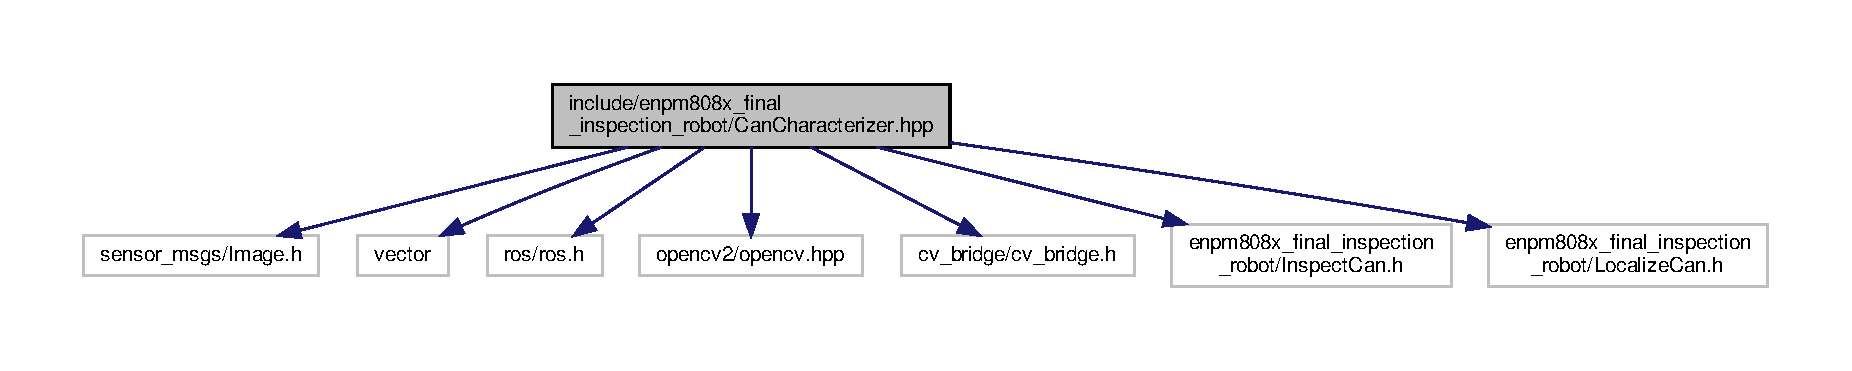
\includegraphics[width=350pt]{CanCharacterizer_8hpp__incl}
\end{center}
\end{figure}
This graph shows which files directly or indirectly include this file\+:\nopagebreak
\begin{figure}[H]
\begin{center}
\leavevmode
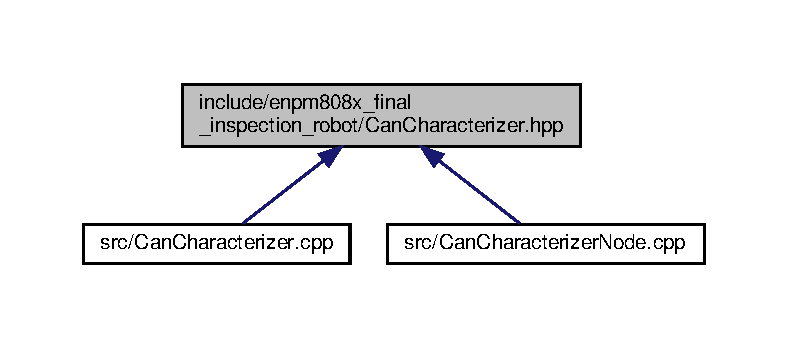
\includegraphics[width=350pt]{CanCharacterizer_8hpp__dep__incl}
\end{center}
\end{figure}
\subsection*{Classes}
\begin{DoxyCompactItemize}
\item 
class \hyperlink{classCanCharacterizer}{Can\+Characterizer}
\begin{DoxyCompactList}\small\item\em The class concerned with the Detection and Localization of the can in front of the T\+I\+A\+Go using two services. \end{DoxyCompactList}\end{DoxyCompactItemize}


\subsection{Detailed Description}
The Class which handles the inspection (Detection) and localization of the Cans present in front of T\+I\+A\+Go in each iteration. 

\begin{DoxyAuthor}{Author}
Aditya Jadhav 
\end{DoxyAuthor}
\begin{DoxyVersion}{Version}
0.\+1 
\end{DoxyVersion}
\begin{DoxyDate}{Date}
2021-\/12-\/05
\end{DoxyDate}
\begin{DoxyCopyright}{Copyright}
Copyright 2021 Robert Vandemark, Aditya Jadhav, Abhishek Nalawade
\end{DoxyCopyright}
Licensed under the Apache License, Version 2.\+0 (the \char`\"{}\+License\char`\"{}); you may not use this file except in compliance with the License. You may obtain a copy of the License at \begin{DoxyVerb}  http://www.apache.org/licenses/LICENSE-2.0
\end{DoxyVerb}


Unless required by applicable law or agreed to in writing, software distributed under the License is distributed on an \char`\"{}\+A\+S I\+S\char`\"{} B\+A\+S\+IS, W\+I\+T\+H\+O\+UT W\+A\+R\+R\+A\+N\+T\+I\+ES OR C\+O\+N\+D\+I\+T\+I\+O\+NS OF A\+NY K\+I\+ND, either express or implied. See the License for the specific language governing permissions and limitations under the License. 
\hypertarget{InspectionController_8hpp}{}\section{include/enpm808x\+\_\+final\+\_\+inspection\+\_\+robot/\+Inspection\+Controller.hpp File Reference}
\label{InspectionController_8hpp}\index{include/enpm808x\+\_\+final\+\_\+inspection\+\_\+robot/\+Inspection\+Controller.\+hpp@{include/enpm808x\+\_\+final\+\_\+inspection\+\_\+robot/\+Inspection\+Controller.\+hpp}}


The main controller for the inspection process pipeline, which helps to communicate objectives and status on the R\+OS network.  


{\ttfamily \#include $<$ros/service\+\_\+client.\+h$>$}\newline
{\ttfamily \#include $<$ros/subscriber.\+h$>$}\newline
{\ttfamily \#include $<$actionlib/client/simple\+\_\+action\+\_\+client.\+h$>$}\newline
{\ttfamily \#include $<$actionlib/client/simple\+\_\+client\+\_\+goal\+\_\+state.\+h$>$}\newline
{\ttfamily \#include $<$move\+\_\+base\+\_\+msgs/\+Move\+Base\+Action.\+h$>$}\newline
{\ttfamily \#include $<$sensor\+\_\+msgs/\+Image.\+h$>$}\newline
{\ttfamily \#include $<$sensor\+\_\+msgs/\+Point\+Cloud2.\+h$>$}\newline
{\ttfamily \#include $<$control\+\_\+msgs/\+Follow\+Joint\+Trajectory\+Action\+Result.\+h$>$}\newline
{\ttfamily \#include $<$tf/transform\+\_\+listener.\+h$>$}\newline
{\ttfamily \#include $<$tf/\+Linear\+Math/\+Transform.\+h$>$}\newline
{\ttfamily \#include $<$tf/\+Linear\+Math/\+Vector3.\+h$>$}\newline
{\ttfamily \#include $<$memory$>$}\newline
{\ttfamily \#include $<$queue$>$}\newline
{\ttfamily \#include $<$vector$>$}\newline
{\ttfamily \#include \char`\"{}enpm808x\+\_\+final\+\_\+inspection\+\_\+robot/\+Inspection\+Metrics.\+h\char`\"{}}\newline
Include dependency graph for Inspection\+Controller.\+hpp\+:\nopagebreak
\begin{figure}[H]
\begin{center}
\leavevmode
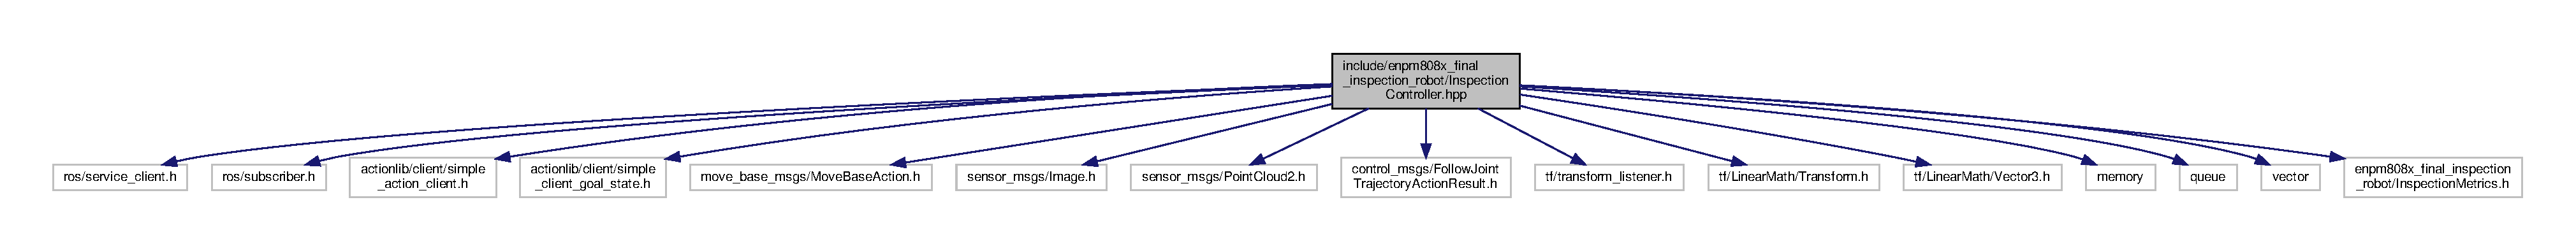
\includegraphics[width=350pt]{InspectionController_8hpp__incl}
\end{center}
\end{figure}
This graph shows which files directly or indirectly include this file\+:\nopagebreak
\begin{figure}[H]
\begin{center}
\leavevmode
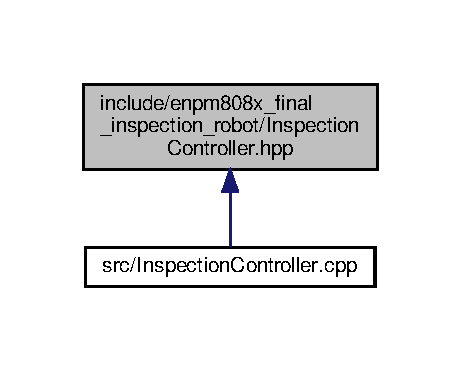
\includegraphics[width=221pt]{InspectionController_8hpp__dep__incl}
\end{center}
\end{figure}
\subsection*{Classes}
\begin{DoxyCompactItemize}
\item 
class \hyperlink{classInspectionController}{Inspection\+Controller}
\end{DoxyCompactItemize}
\subsection*{Typedefs}
\begin{DoxyCompactItemize}
\item 
\mbox{\Hypertarget{InspectionController_8hpp_ad9d82b56812eee6c9be862194f37f663}\label{InspectionController_8hpp_ad9d82b56812eee6c9be862194f37f663}} 
{\footnotesize template$<$typename T $>$ }\\using {\bfseries uptr} = std\+::unique\+\_\+ptr$<$ T $>$
\item 
\mbox{\Hypertarget{InspectionController_8hpp_adc49b550c7d757bf32374d4b89eaa000}\label{InspectionController_8hpp_adc49b550c7d757bf32374d4b89eaa000}} 
using {\bfseries Move\+Base\+Action\+Cli} = actionlib\+::\+Simple\+Action\+Client$<$ move\+\_\+base\+\_\+msgs\+::\+Move\+Base\+Action $>$
\end{DoxyCompactItemize}


\subsection{Detailed Description}
The main controller for the inspection process pipeline, which helps to communicate objectives and status on the R\+OS network. 

\begin{DoxyAuthor}{Author}
Robert Vandemark 
\end{DoxyAuthor}
\begin{DoxyVersion}{Version}
0.\+1 
\end{DoxyVersion}
\begin{DoxyDate}{Date}
2021-\/12-\/05
\end{DoxyDate}
\begin{DoxyCopyright}{Copyright}
Copyright 2021 Robert Vandemark, Aditya Jadhav, Abhishek Nalawade
\end{DoxyCopyright}
Licensed under the Apache License, Version 2.\+0 (the \char`\"{}\+License\char`\"{}); you may not use this file except in compliance with the License. You may obtain a copy of the License at \begin{DoxyVerb}  http://www.apache.org/licenses/LICENSE-2.0
\end{DoxyVerb}


Unless required by applicable law or agreed to in writing, software distributed under the License is distributed on an \char`\"{}\+A\+S I\+S\char`\"{} B\+A\+S\+IS, W\+I\+T\+H\+O\+UT W\+A\+R\+R\+A\+N\+T\+I\+ES OR C\+O\+N\+D\+I\+T\+I\+O\+NS OF A\+NY K\+I\+ND, either express or implied. See the License for the specific language governing permissions and limitations under the License. 
\hypertarget{CanCharacterizer_8cpp}{}\section{src/\+Can\+Characterizer.cpp File Reference}
\label{CanCharacterizer_8cpp}\index{src/\+Can\+Characterizer.\+cpp@{src/\+Can\+Characterizer.\+cpp}}


The Class which handles the inspection (Detection) and localization of the Cans present in front of T\+I\+A\+Go in each iteration.  


{\ttfamily \#include \char`\"{}enpm808x\+\_\+final\+\_\+inspection\+\_\+robot/\+Can\+Characterizer.\+hpp\char`\"{}}\newline
Include dependency graph for Can\+Characterizer.\+cpp\+:\nopagebreak
\begin{figure}[H]
\begin{center}
\leavevmode
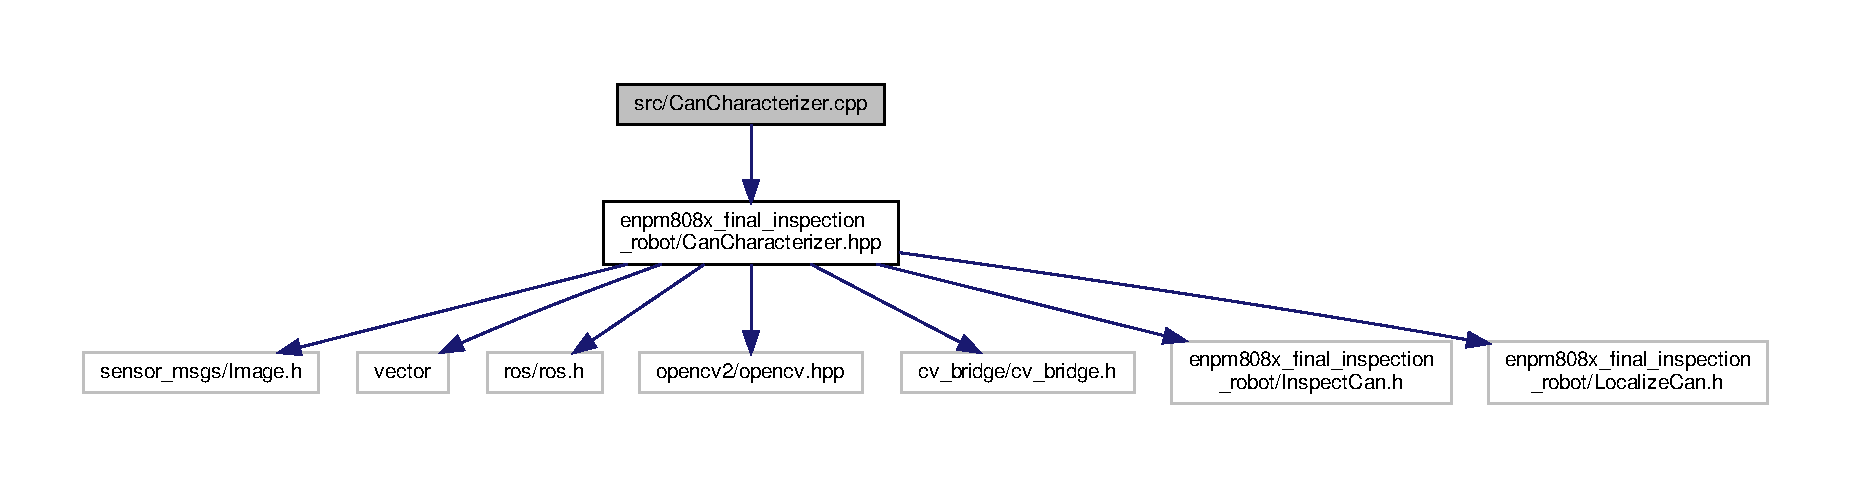
\includegraphics[width=350pt]{CanCharacterizer_8cpp__incl}
\end{center}
\end{figure}


\subsection{Detailed Description}
The Class which handles the inspection (Detection) and localization of the Cans present in front of T\+I\+A\+Go in each iteration. 

\begin{DoxyAuthor}{Author}
Aditya Jadhav 
\end{DoxyAuthor}
\begin{DoxyVersion}{Version}
0.\+1 
\end{DoxyVersion}
\begin{DoxyDate}{Date}
2021-\/12-\/05
\end{DoxyDate}
\begin{DoxyCopyright}{Copyright}
Copyright 2021 Robert Vandemark, Aditya Jadhav, Abhishek Nalawade
\end{DoxyCopyright}
Licensed under the Apache License, Version 2.\+0 (the \char`\"{}\+License\char`\"{}); you may not use this file except in compliance with the License. You may obtain a copy of the License at \begin{DoxyVerb}  http://www.apache.org/licenses/LICENSE-2.0
\end{DoxyVerb}


Unless required by applicable law or agreed to in writing, software distributed under the License is distributed on an \char`\"{}\+A\+S I\+S\char`\"{} B\+A\+S\+IS, W\+I\+T\+H\+O\+UT W\+A\+R\+R\+A\+N\+T\+I\+ES OR C\+O\+N\+D\+I\+T\+I\+O\+NS OF A\+NY K\+I\+ND, either express or implied. See the License for the specific language governing permissions and limitations under the License. 
\hypertarget{CanCharacterizerNode_8cpp}{}\section{src/\+Can\+Characterizer\+Node.cpp File Reference}
\label{CanCharacterizerNode_8cpp}\index{src/\+Can\+Characterizer\+Node.\+cpp@{src/\+Can\+Characterizer\+Node.\+cpp}}


The node used for inspection and localization of the Can.  


{\ttfamily \#include \char`\"{}ros/ros.\+h\char`\"{}}\newline
{\ttfamily \#include \char`\"{}enpm808x\+\_\+final\+\_\+inspection\+\_\+robot/\+Can\+Characterizer.\+hpp\char`\"{}}\newline
Include dependency graph for Can\+Characterizer\+Node.\+cpp\+:\nopagebreak
\begin{figure}[H]
\begin{center}
\leavevmode
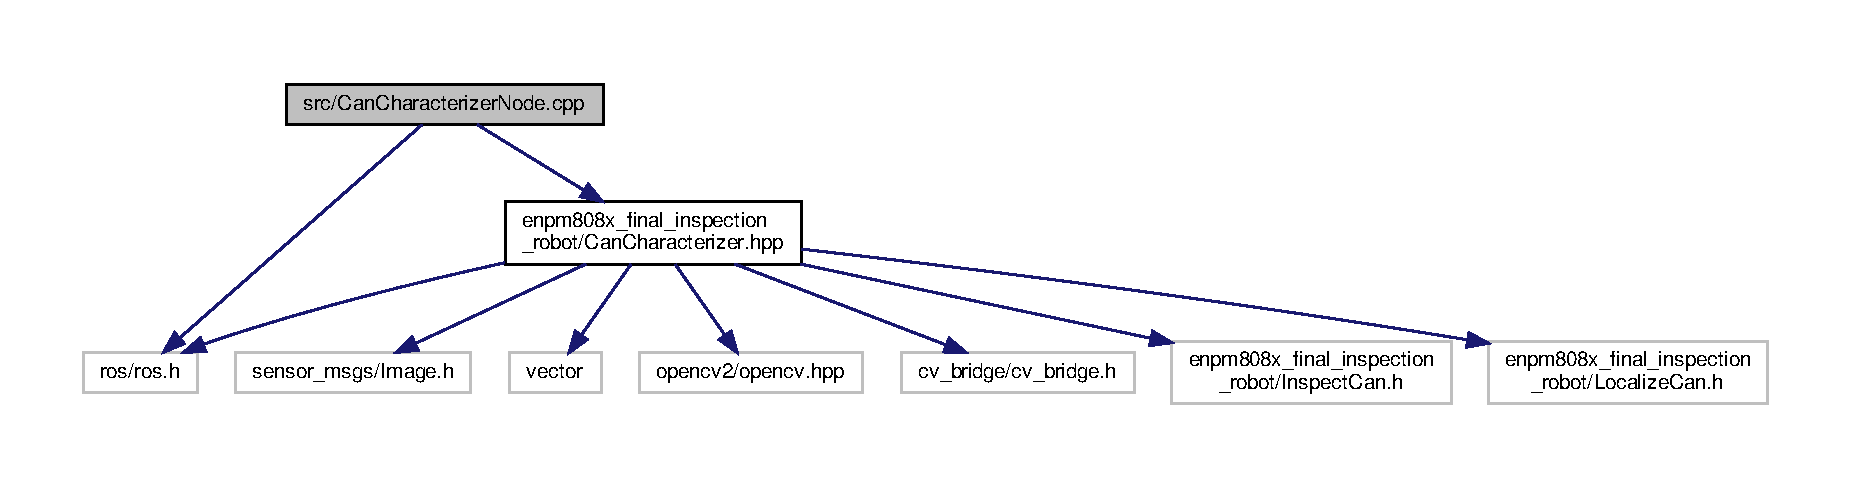
\includegraphics[width=350pt]{CanCharacterizerNode_8cpp__incl}
\end{center}
\end{figure}
\subsection*{Functions}
\begin{DoxyCompactItemize}
\item 
\mbox{\Hypertarget{CanCharacterizerNode_8cpp_a3c04138a5bfe5d72780bb7e82a18e627}\label{CanCharacterizerNode_8cpp_a3c04138a5bfe5d72780bb7e82a18e627}} 
int \hyperlink{CanCharacterizerNode_8cpp_a3c04138a5bfe5d72780bb7e82a18e627}{main} (int argc, char $\ast$$\ast$argv)
\begin{DoxyCompactList}\small\item\em Inspector Node overseeing the Can Detection and Localization. \end{DoxyCompactList}\end{DoxyCompactItemize}


\subsection{Detailed Description}
The node used for inspection and localization of the Can. 

\begin{DoxyAuthor}{Author}
Aditya Jadhav 
\end{DoxyAuthor}
\begin{DoxyVersion}{Version}
0.\+1 
\end{DoxyVersion}
\begin{DoxyDate}{Date}
2021-\/12-\/05
\end{DoxyDate}
\begin{DoxyCopyright}{Copyright}
Copyright 2021 Robert Vandemark, Aditya Jadhav, Abhishek Nalawade
\end{DoxyCopyright}
Licensed under the Apache License, Version 2.\+0 (the \char`\"{}\+License\char`\"{}); you may not use this file except in compliance with the License. You may obtain a copy of the License at \begin{DoxyVerb}  http://www.apache.org/licenses/LICENSE-2.0
\end{DoxyVerb}


Unless required by applicable law or agreed to in writing, software distributed under the License is distributed on an \char`\"{}\+A\+S I\+S\char`\"{} B\+A\+S\+IS, W\+I\+T\+H\+O\+UT W\+A\+R\+R\+A\+N\+T\+I\+ES OR C\+O\+N\+D\+I\+T\+I\+O\+NS OF A\+NY K\+I\+ND, either express or implied. See the License for the specific language governing permissions and limitations under the License. 
\hypertarget{InspectionController_8cpp}{}\section{src/\+Inspection\+Controller.cpp File Reference}
\label{InspectionController_8cpp}\index{src/\+Inspection\+Controller.\+cpp@{src/\+Inspection\+Controller.\+cpp}}


The main controller for the inspection process pipeline, which helps to communicate objectives and status on the R\+OS network.  


{\ttfamily \#include \char`\"{}enpm808x\+\_\+final\+\_\+inspection\+\_\+robot/\+Inspection\+Controller.\+hpp\char`\"{}}\newline
Include dependency graph for Inspection\+Controller.\+cpp\+:\nopagebreak
\begin{figure}[H]
\begin{center}
\leavevmode
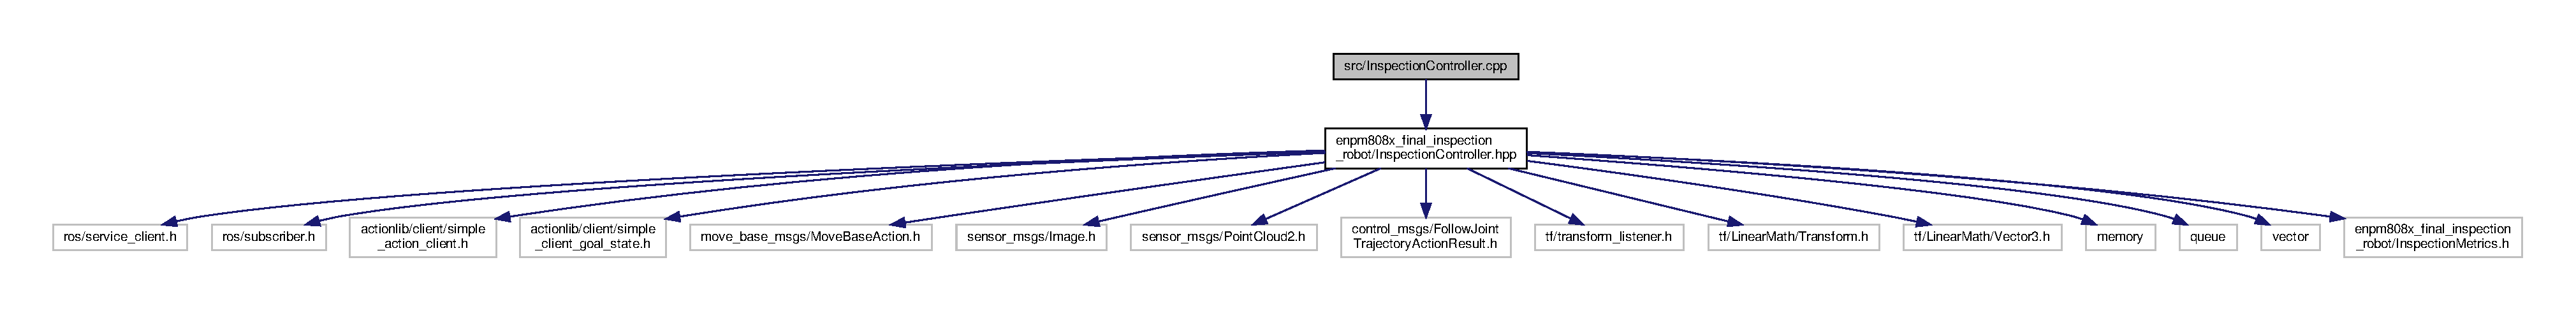
\includegraphics[width=350pt]{InspectionController_8cpp__incl}
\end{center}
\end{figure}


\subsection{Detailed Description}
The main controller for the inspection process pipeline, which helps to communicate objectives and status on the R\+OS network. 

\begin{DoxyAuthor}{Author}
Robert Vandemark 
\end{DoxyAuthor}
\begin{DoxyVersion}{Version}
0.\+1 
\end{DoxyVersion}
\begin{DoxyDate}{Date}
2021-\/12-\/05
\end{DoxyDate}
\begin{DoxyCopyright}{Copyright}
Copyright 2021 Robert Vandemark, Aditya Jadhav, Abhishek Nalawade
\end{DoxyCopyright}
Licensed under the Apache License, Version 2.\+0 (the \char`\"{}\+License\char`\"{}); you may not use this file except in compliance with the License. You may obtain a copy of the License at \begin{DoxyVerb}  http://www.apache.org/licenses/LICENSE-2.0
\end{DoxyVerb}


Unless required by applicable law or agreed to in writing, software distributed under the License is distributed on an \char`\"{}\+A\+S I\+S\char`\"{} B\+A\+S\+IS, W\+I\+T\+H\+O\+UT W\+A\+R\+R\+A\+N\+T\+I\+ES OR C\+O\+N\+D\+I\+T\+I\+O\+NS OF A\+NY K\+I\+ND, either express or implied. See the License for the specific language governing permissions and limitations under the License. 
\hypertarget{InspectionControllerNode_8cpp}{}\section{src/\+Inspection\+Controller\+Node.cpp File Reference}
\label{InspectionControllerNode_8cpp}\index{src/\+Inspection\+Controller\+Node.\+cpp@{src/\+Inspection\+Controller\+Node.\+cpp}}


The node encapsulating the inspection process\textquotesingle{}s main controller.  


\subsection*{Functions}
\begin{DoxyCompactItemize}
\item 
int \hyperlink{InspectionControllerNode_8cpp_a3c04138a5bfe5d72780bb7e82a18e627}{main} (int argc, char $\ast$$\ast$argv)
\end{DoxyCompactItemize}


\subsection{Detailed Description}
The node encapsulating the inspection process\textquotesingle{}s main controller. 

\begin{DoxyAuthor}{Author}
Robert Vandemark 
\end{DoxyAuthor}
\begin{DoxyVersion}{Version}
0.\+1 
\end{DoxyVersion}
\begin{DoxyDate}{Date}
2021-\/12-\/05
\end{DoxyDate}
\begin{DoxyCopyright}{Copyright}
Copyright 2021 Robert Vandemark, Aditya Jadhav, Abhishek Nalawade
\end{DoxyCopyright}
Licensed under the Apache License, Version 2.\+0 (the \char`\"{}\+License\char`\"{}); you may not use this file except in compliance with the License. You may obtain a copy of the License at \begin{DoxyVerb}  http://www.apache.org/licenses/LICENSE-2.0
\end{DoxyVerb}


Unless required by applicable law or agreed to in writing, software distributed under the License is distributed on an \char`\"{}\+A\+S I\+S\char`\"{} B\+A\+S\+IS, W\+I\+T\+H\+O\+UT W\+A\+R\+R\+A\+N\+T\+I\+ES OR C\+O\+N\+D\+I\+T\+I\+O\+NS OF A\+NY K\+I\+ND, either express or implied. See the License for the specific language governing permissions and limitations under the License. 

\subsection{Function Documentation}
\mbox{\Hypertarget{InspectionControllerNode_8cpp_a3c04138a5bfe5d72780bb7e82a18e627}\label{InspectionControllerNode_8cpp_a3c04138a5bfe5d72780bb7e82a18e627}} 
\index{Inspection\+Controller\+Node.\+cpp@{Inspection\+Controller\+Node.\+cpp}!main@{main}}
\index{main@{main}!Inspection\+Controller\+Node.\+cpp@{Inspection\+Controller\+Node.\+cpp}}
\subsubsection{\texorpdfstring{main()}{main()}}
{\footnotesize\ttfamily int main (\begin{DoxyParamCaption}\item[{int}]{argc,  }\item[{char $\ast$$\ast$}]{argv }\end{DoxyParamCaption})}

The main entry point of our inspection controller node. 
\begin{DoxyParams}{Parameters}
{\em argc} & The number of program arguments. \\
\hline
{\em argv} & The list of program argument strings. \\
\hline
\end{DoxyParams}
\begin{DoxyReturn}{Returns}
The return code of the node\textquotesingle{}s operation. 
\end{DoxyReturn}

\hypertarget{TestMain_8cpp}{}\section{test/\+Test\+Main.cpp File Reference}
\label{TestMain_8cpp}\index{test/\+Test\+Main.\+cpp@{test/\+Test\+Main.\+cpp}}


The testing suite\textquotesingle{}s entry point.  


{\ttfamily \#include $<$ros/ros.\+h$>$}\newline
{\ttfamily \#include $<$ros/package.\+h$>$}\newline
{\ttfamily \#include $<$gtest/gtest.\+h$>$}\newline
{\ttfamily \#include $<$sensor\+\_\+msgs/image\+\_\+encodings.\+h$>$}\newline
{\ttfamily \#include $<$memory$>$}\newline
{\ttfamily \#include $<$string$>$}\newline
{\ttfamily \#include $<$opencv2/opencv.\+hpp$>$}\newline
{\ttfamily \#include \char`\"{}cv\+\_\+bridge/cv\+\_\+bridge.\+h\char`\"{}}\newline
{\ttfamily \#include \char`\"{}enpm808x\+\_\+final\+\_\+inspection\+\_\+robot/\+Localize\+Can.\+h\char`\"{}}\newline
{\ttfamily \#include \char`\"{}enpm808x\+\_\+final\+\_\+inspection\+\_\+robot/\+Inspect\+Can.\+h\char`\"{}}\newline
Include dependency graph for Test\+Main.\+cpp\+:\nopagebreak
\begin{figure}[H]
\begin{center}
\leavevmode
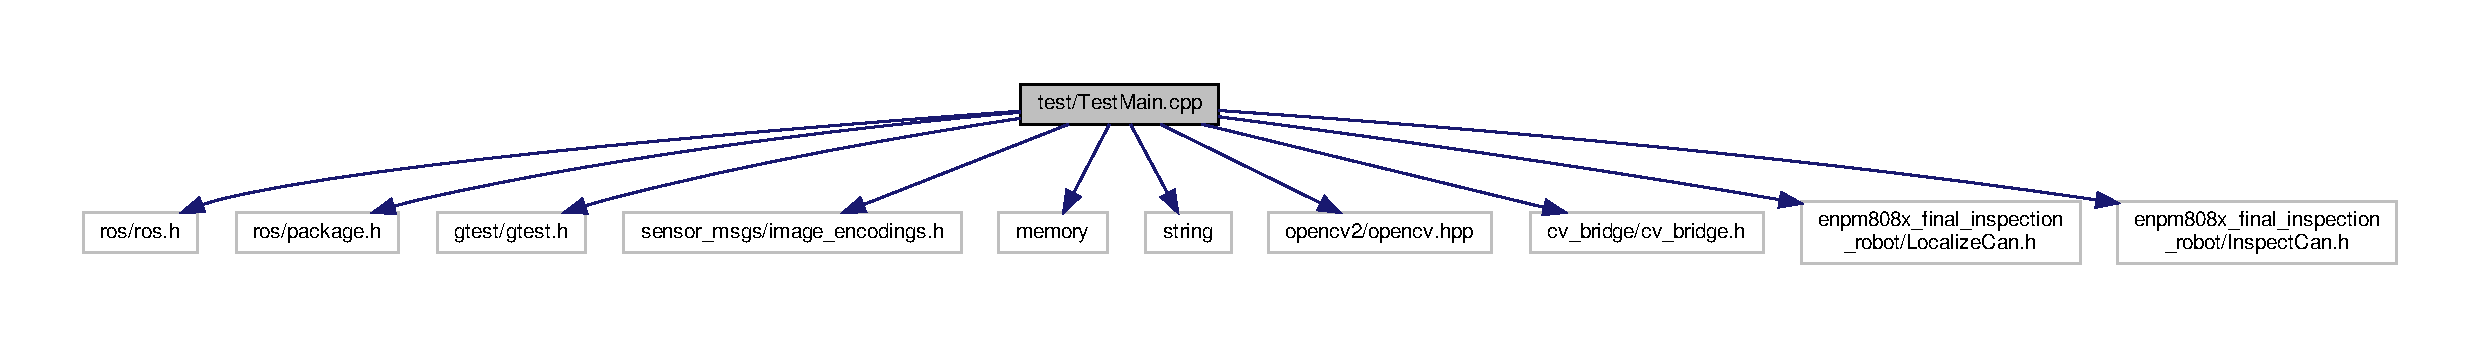
\includegraphics[width=350pt]{TestMain_8cpp__incl}
\end{center}
\end{figure}
\subsection*{Functions}
\begin{DoxyCompactItemize}
\item 
\hyperlink{TestMain_8cpp_a22715320dea6bd3070869d1ff04f398a}{T\+E\+ST} (Inspect\+Can\+Test, Test\+\_\+\+Inspect\+\_\+can)
\item 
\hyperlink{TestMain_8cpp_a4de53239e0168ea2bf104003f13f9fc2}{T\+E\+ST} (Handle\+\_\+\+Inspect\+Can, Test\+\_\+\+Inspection\+Can\+\_\+callback)
\item 
\mbox{\Hypertarget{TestMain_8cpp_a26e30743d23b8ec75c157a2f238e85fb}\label{TestMain_8cpp_a26e30743d23b8ec75c157a2f238e85fb}} 
{\bfseries T\+E\+ST} (T\+E\+S\+T\+Suite, test\+Main)
\item 
\hyperlink{TestMain_8cpp_a018004d92704a8a93a524515062ba98b}{T\+E\+ST} (Localize\+Can\+Test, Test\+\_\+\+Localize\+Can\+\_\+\+Existence)
\item 
\mbox{\Hypertarget{TestMain_8cpp_a3c04138a5bfe5d72780bb7e82a18e627}\label{TestMain_8cpp_a3c04138a5bfe5d72780bb7e82a18e627}} 
int {\bfseries main} (int argc, char $\ast$$\ast$argv)
\end{DoxyCompactItemize}
\subsection*{Variables}
\begin{DoxyCompactItemize}
\item 
\mbox{\Hypertarget{TestMain_8cpp_afbb7c6b17cf5b1463c6d18f09e6eb70e}\label{TestMain_8cpp_afbb7c6b17cf5b1463c6d18f09e6eb70e}} 
std\+::unique\+\_\+ptr$<$ ros\+::\+Node\+Handle $>$ {\bfseries nh}
\end{DoxyCompactItemize}


\subsection{Detailed Description}
The testing suite\textquotesingle{}s entry point. 

\begin{DoxyAuthor}{Author}
Robert Vandemark 
\end{DoxyAuthor}
\begin{DoxyVersion}{Version}
0.\+1 
\end{DoxyVersion}
\begin{DoxyDate}{Date}
2021-\/12-\/06
\end{DoxyDate}
\begin{DoxyCopyright}{Copyright}
Copyright 2021 Robert Vandemark, Aditya Jadhav, Abhishek Nalawade
\end{DoxyCopyright}
Licensed under the Apache License, Version 2.\+0 (the \char`\"{}\+License\char`\"{}); you may not use this file except in compliance with the License. You may obtain a copy of the License at \begin{DoxyVerb}  http://www.apache.org/licenses/LICENSE-2.0
\end{DoxyVerb}


Unless required by applicable law or agreed to in writing, software distributed under the License is distributed on an \char`\"{}\+A\+S I\+S\char`\"{} B\+A\+S\+IS, W\+I\+T\+H\+O\+UT W\+A\+R\+R\+A\+N\+T\+I\+ES OR C\+O\+N\+D\+I\+T\+I\+O\+NS OF A\+NY K\+I\+ND, either express or implied. See the License for the specific language governing permissions and limitations under the License. 

\subsection{Function Documentation}
\mbox{\Hypertarget{TestMain_8cpp_a22715320dea6bd3070869d1ff04f398a}\label{TestMain_8cpp_a22715320dea6bd3070869d1ff04f398a}} 
\index{Test\+Main.\+cpp@{Test\+Main.\+cpp}!T\+E\+ST@{T\+E\+ST}}
\index{T\+E\+ST@{T\+E\+ST}!Test\+Main.\+cpp@{Test\+Main.\+cpp}}
\subsubsection{\texorpdfstring{T\+E\+S\+T()}{TEST()}\hspace{0.1cm}{\footnotesize\ttfamily [1/3]}}
{\footnotesize\ttfamily T\+E\+ST (\begin{DoxyParamCaption}\item[{Inspect\+Can\+Test}]{,  }\item[{Test\+\_\+\+Inspect\+\_\+can}]{ }\end{DoxyParamCaption})}

Simple Existence Test for the Inspect\+Can Service. \mbox{\Hypertarget{TestMain_8cpp_a4de53239e0168ea2bf104003f13f9fc2}\label{TestMain_8cpp_a4de53239e0168ea2bf104003f13f9fc2}} 
\index{Test\+Main.\+cpp@{Test\+Main.\+cpp}!T\+E\+ST@{T\+E\+ST}}
\index{T\+E\+ST@{T\+E\+ST}!Test\+Main.\+cpp@{Test\+Main.\+cpp}}
\subsubsection{\texorpdfstring{T\+E\+S\+T()}{TEST()}\hspace{0.1cm}{\footnotesize\ttfamily [2/3]}}
{\footnotesize\ttfamily T\+E\+ST (\begin{DoxyParamCaption}\item[{Handle\+\_\+\+Inspect\+Can}]{,  }\item[{Test\+\_\+\+Inspection\+Can\+\_\+callback}]{ }\end{DoxyParamCaption})}

Testing the inspect can service callback function handle\+Inspect\+Can\+Request \mbox{\Hypertarget{TestMain_8cpp_a018004d92704a8a93a524515062ba98b}\label{TestMain_8cpp_a018004d92704a8a93a524515062ba98b}} 
\index{Test\+Main.\+cpp@{Test\+Main.\+cpp}!T\+E\+ST@{T\+E\+ST}}
\index{T\+E\+ST@{T\+E\+ST}!Test\+Main.\+cpp@{Test\+Main.\+cpp}}
\subsubsection{\texorpdfstring{T\+E\+S\+T()}{TEST()}\hspace{0.1cm}{\footnotesize\ttfamily [3/3]}}
{\footnotesize\ttfamily T\+E\+ST (\begin{DoxyParamCaption}\item[{Localize\+Can\+Test}]{,  }\item[{Test\+\_\+\+Localize\+Can\+\_\+\+Existence}]{ }\end{DoxyParamCaption})}

Simple Existence Test for the Localize\+Can Service. 
%--- End generated contents ---

% Index
\backmatter
\newpage
\phantomsection
\clearemptydoublepage
\addcontentsline{toc}{chapter}{Index}
\printindex

\end{document}
